\documentclass[14pt]{extarticle}
\usepackage{graphicx}
\usepackage[T1]{fontenc} 
\usepackage[margin=1in]{geometry}
\usepackage{hyperref}

% Custom captions: 1 pav.
\usepackage{caption}
\captionsetup[figure]{labelformat=empty}
\renewcommand{\thefigure}{\arabic{figure} pav.}

% Turinys vietoj Contents
\renewcommand{\contentsname}{Turinys}

\begin{document}

% Titulinis
\begin{titlepage}
	\begin{center}
		
\includegraphics[width=5cm]{images/ktu_logo.png}

		\textbf{Kauno technologijos universitetas}

		Informatikos fakultetas

		\vspace{3cm}

		\textbf{Individualus darbas}

		\vspace{0.5cm}
		P175B120 Paslaugų programavimas debesų kompiuterijoje

	\end{center}

	\begin{flushright}

		\vfill

		\textbf{Arnas Bradauskas}

		Studentas

		\vspace{0.2cm}

		\textbf{Doc. Vytautas Pilkauskas}

		Dėstytojas

	\end{flushright}

	\begin{center}
		Kaunas, 2024
	\end{center}

\end{titlepage}

% Turinys
\tableofcontents

\clearpage

\section{Pridėti mikroservisai}

Nebuvo pridėta mikroservisų

\clearpage

\section{Paleidimas lokaliame kubernetes klasteryje}

Sukurti 4 servisai - studentsapi, coursesapi, apigateway ir db.

Failo pavyzdys:

\begin{verbatim}
apiVersion: apps/v1
kind: Deployment
metadata:
  name: test
spec:
  replicas: 1
  selector:
    matchLabels:
      app: test
  template:
    metadata:
      labels:
        app: test
    spec:
      containers:
      - name: test
        image: arnasbrad/imageName:latest
        imagePullPolicy: IfNotPresent
        ports:
        - containerPort: 8080
        env:
        - name: ASPNETCORE_ENVIRONMENT
          value: "Development"
        - name: ConnectionStrings__testContext
          value: "<context_string>"

---

apiVersion: v1
kind: Service
metadata:
  name: test
spec:
  type: ClusterIP
  ports:
  - port: 8080
    targetPort: 8080
  selector:
    app: test
\end{verbatim}

Pagal šį šabloną sukurti yaml deployment failai.

Su šia komanda sukeliame pods ir services į klasterį.
\begin{verbatim}
kubectl apply -f deploymentsDirectory
\end{verbatim}

Visus failus galima rasti čia: \href{https://github.com/arnasbrad/clouds_inz}{GitHub repozitorija}

\clearpage
Rezultatai:

\begin{figure}[!htbp]
	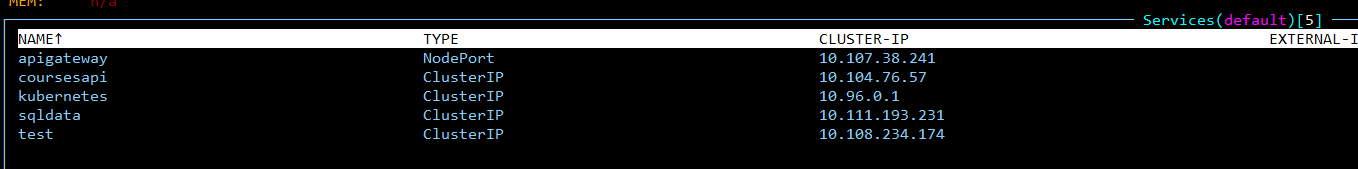
\includegraphics[width=\textwidth]{images/first/1.png}
	\caption{\thefigure\ K9s matomi services.}
\end{figure}

\begin{figure}[!htbp]
	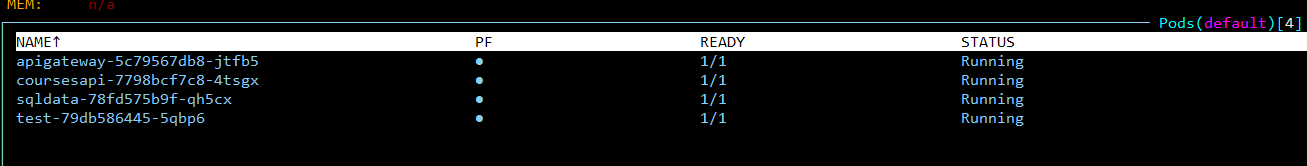
\includegraphics[width=\textwidth]{images/first/2.png}
	\caption{\thefigure\ K9s matomi pods.}
\end{figure}

\begin{figure}[!htbp]
	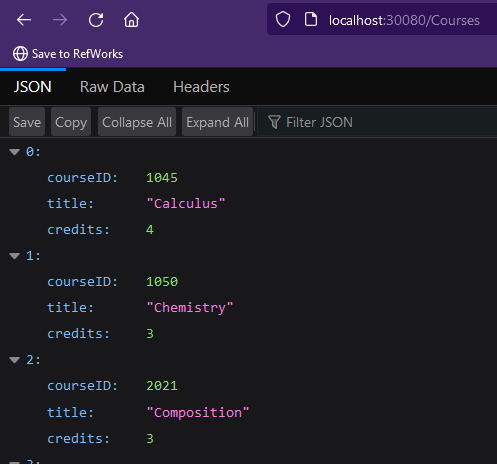
\includegraphics[width=\textwidth]{images/first/3.png}
	\caption{\thefigure\ Pasiektas CoursesApi per ApiGateway.}
\end{figure}

\begin{figure}[!htbp]
	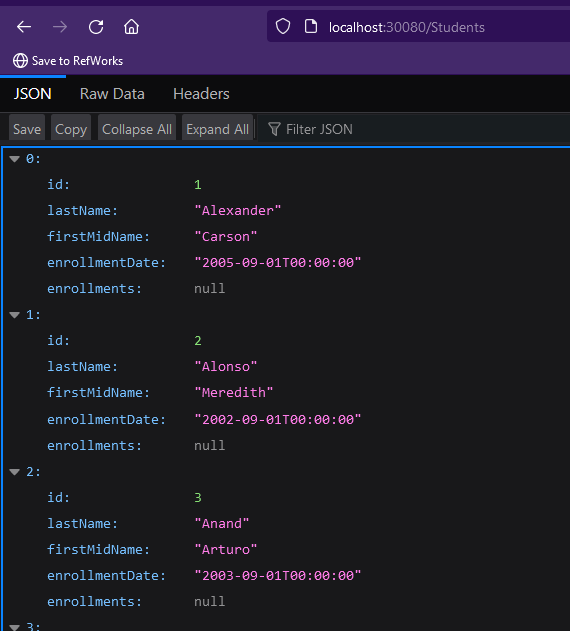
\includegraphics[width=\textwidth]{images/first/4.png}
	\caption{\thefigure\ Pasiektas StudentsApi per ApiGateway.}
\end{figure}

\begin{figure}[!htbp]
	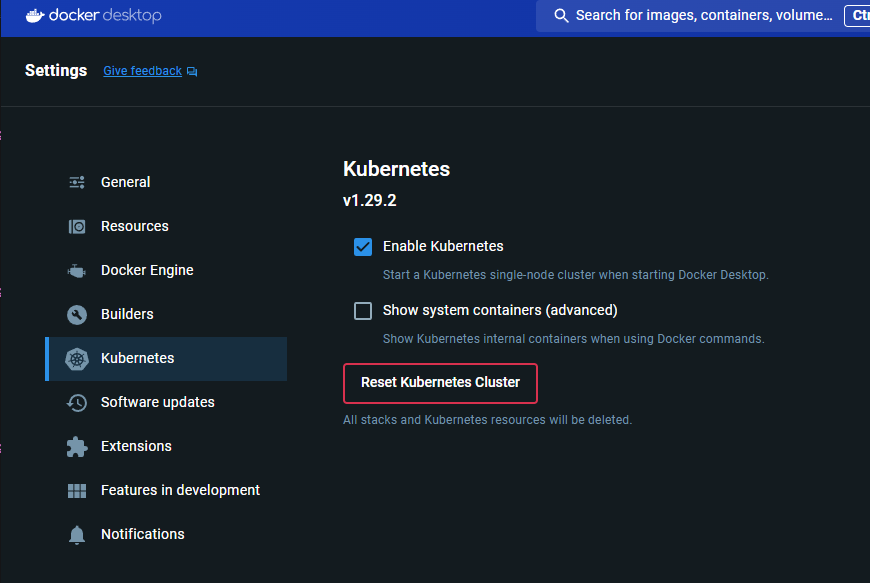
\includegraphics[width=\textwidth]{images/first/5.png}
	\caption{\thefigure\ Naudotas klasteris (docker desktop).}
\end{figure}

\clearpage

\end{document}
